\documentclass[conference]{IEEEtran}
\IEEEoverridecommandlockouts
% The preceding line is only needed to identify funding in the first footnote. If that is unneeded, please comment it out.
%Template version as of 6/27/2024

\usepackage{cite}
\usepackage{amsmath,amssymb,amsfonts}
\usepackage{algorithmic}
\usepackage{graphicx}
\usepackage{textcomp}
\usepackage{xcolor}
\def\BibTeX{{\rm B\kern-.05em{\sc i\kern-.025em b}\kern-.08em
    T\kern-.1667em\lower.7ex\hbox{E}\kern-.125emX}}
\def\IEEEkeywordsname{Keywords}
\begin{document}

\title{Counterfactual Simulation of Extreme Mental Health Scenarios for Clinical Preparedness via Fine-Tuned LLMs and Explainable AI}

\author{
\begin{tabular}{ccc}
{Gangavarapu Lakshmi Dhatri} & {Kumari Khushi Singh} & {Likitha C} \\
\textit{Dept. of CSE, REVA University} & \textit{Dept. of CSE, REVA University} & \textit{Dept. of CSE, REVA University} \\
Bengaluru, India & Bengaluru, India & Bengaluru, India \\
lakshmidhatri.gangavarapu@gmail.com & kumari.khushi.singh@gmail.com & likithaanuchandru@gmail.com \\
\end{tabular}

\\
\\

\begin{tabular}{cc}
{Harshitha N} & {Dr. Priyanka Bharti} \\
\textit{Dept. of CSE, REVA University} & \textit{Dept. of CSE, REVA University} \\
Bengaluru, India & Bengaluru, India \\
harshithamurthy31@gmail.com & priyanka.bharti@reva.edu.in \\
\end{tabular}
}

\maketitle

\begin{abstract}
Clinical notes on patients with mental health conditions contain rich, unstructured information that remains critically underutilized in clinical decision-making. Existing AI systems for mental health prioritize risk score prediction, leaving clinicians unprepared for extreme adverse patient trajectories. We propose and implement a fine-tuned large language model (LLM) framework with post-hoc explainability that acts as a second reader of mental health documentation---not to predict outcomes, but to prepare clinicians for extreme patient trajectories. The framework operates through a multi-stage pipeline: (1)~Clinical Factor Extraction using a LoRA-adapted Microsoft Phi-3.5-Mini-Instruct model with DSM-5/ICD-11 grounded schema; (2)~Post-Extraction Validation including ICD code normalization, context enrichment for housing/trauma/functional decline, and negation-aware critical signal detection; (3)~Evidence-Based Branch Gating that conditionally executes scenario pathways only when clinical evidence exists; (4)~Tree-of-Thoughts Scenario Generation across three escalation pathways (psychiatric deterioration, substance use, social collapse); (5)~Clinical Report Generation with consistency checking and severity inference; and (6)~Counterfactual Evidence Attribution, an explainable AI layer that maps each generated scenario trigger back to specific text spans in the original clinical note with color-coded highlighting and nexus factor detection. The system is trained on 94,592 de-identified discharge summaries from MIMIC-IV, achieving evaluation loss of 1.706 and 67.5\% mean token accuracy. We present the complete architecture, training methodology, and qualitative analysis demonstrating grounded counterfactual generation with interpretable evidence trails.
\end{abstract}

\begin{IEEEkeywords}
counterfactual reasoning, mental health, large language models, clinical NLP, explainable AI, evidence attribution, clinical decision support, scenario simulation, DSM-5.
\end{IEEEkeywords}

\section{Introduction}

Mental health disorders represent one of the leading causes of disability worldwide, with depression, anxiety, and substance use disorders affecting hundreds of millions of individuals globally \cite{b1}. Clinical documentation, particularly discharge summaries, captures rich longitudinal patient information including symptom progression, treatment history, risk indicators, and psychosocial context. However, this unstructured textual data remains critically underutilized in clinical decision-making \cite{b2}. Natural language processing (NLP) techniques applied to free-text clinical notes have demonstrated significant potential for improving downstream decision quality \cite{b3}, yet existing systems predominantly treat clinical notes as inputs for binary risk scoring rather than as foundations for forward-looking clinical preparedness.

Large language models (LLMs) have emerged as powerful tools for clinical text understanding, with domain-specific fine-tuning shown to substantially improve performance on mental health tasks \cite{b4}, \cite{b5}. Comprehensive reviews of LLMs in mental health care have identified two persistent unresolved challenges: the lack of explainability in model outputs and insufficient alignment with established clinical taxonomies such as DSM-5 and ICD-11 \cite{b6}, \cite{b7}. Critically, all existing LLM-based approaches remain focused on risk classification. None have been proposed as a \textit{second reader} that generates structured narratives of extreme adverse trajectories with traceable evidence attribution.

In this paper, we present the design, implementation, and evaluation of a fine-tuned LLM framework that acts as a second reader of mental health documentation. The framework is designed not to predict outcomes but to prepare clinicians for extreme adverse trajectories, with an explainable AI layer providing evidence trails for every generated scenario. Our contributions are:

\begin{enumerate}
\item A multi-stage pipeline comprising clinical factor extraction, post-extraction validation (ICD normalization, context enrichment, negation-aware signal detection), evidence-based branch gating, Tree-of-Thoughts scenario generation, and clinical report synthesis.
\item A LoRA-adapted Microsoft Phi-3.5-Mini-Instruct model (3.8B parameters) fine-tuned on 94,592 discharge summaries for schema-based clinical factor extraction.
\item A comprehensive safety layer including negation-aware critical signal detection that distinguishes ``threatened suicide'' from ``denies suicidal ideation,'' with automatic risk tier override.
\item A context enrichment module that extracts housing crisis, trauma history, caregiver loss, functional decline, and clinician prognosis statements that the fixed schema cannot capture.
\item Evidence-based branch gating that conditionally skips scenario pathways (e.g., substance use) when no supporting clinical evidence exists, preventing hallucinated scenarios.
\item A counterfactual evidence attribution layer (XAI) that maps each scenario trigger back to specific character spans in the original clinical note, with branch-colored highlighting and nexus factor detection for multi-pathway risk points.
\item Training analysis demonstrating convergence to evaluation loss of 1.706 and 67.5\% mean token accuracy over 35.8 hours on 6 Tesla V100 GPUs.
\end{enumerate}

\section{Related Work}

\subsection{Clinical NLP for Mental Health}

Extracting structured clinical information from unstructured notes is foundational to clinical NLP. Sezgin et al. \cite{b3} demonstrated NLP-based extraction from patient-generated health data. Teferra et al. \cite{b15} found that text-based features contribute more substantially to mental health risk detection than structured markers. Lho et al. \cite{b16} showed LLM-based embeddings achieve strong AUROC for depression and suicide detection. However, these approaches treat notes as inputs for risk scoring rather than structured, schema-driven factor extraction with evidence grounding.

\subsection{LLMs for Mental Health}

Xu et al. \cite{b4} introduced Mental-LLM, demonstrating domain-specific fine-tuning is prerequisite for reliable mental health prediction. Hua et al. \cite{b6} and Guo et al. \cite{b5} identified gaps in safety evaluation and explainability. Kim and Wang \cite{b17} explored DSM-5 grounded hybrid frameworks. Despite advances, no existing system generates structured extreme scenario narratives with traceable evidence attribution.

\subsection{Counterfactual Reasoning in Clinical AI}

Prosperi et al. \cite{b8} articulated the clinical potential of counterfactual AI for simulating rare scenarios. Gat et al. \cite{b9} demonstrated fine-tuned LLMs generate plausible counterfactuals. Chen et al. \cite{b18} found general-purpose LLMs lack depth for high-stakes reasoning. Our framework applies counterfactual simulation specifically to extreme mental health trajectories with post-hoc evidence attribution.

\subsection{Explainability in Clinical AI}

Conventional XAI techniques such as SHAP and LIME have been critiqued for lacking clinical actionability \cite{b10}. Generative XAI frameworks that translate model reasoning into clinical narratives represent an emerging alternative \cite{b11}. Our evidence attribution approach provides post-hoc interpretability by grounding each scenario output in specific input spans---a form of counterfactual traceability rather than feature importance scoring.

\section{Proposed Methodology}

The framework operates as a multi-stage pipeline illustrated in Fig.~\ref{fig:architecture}. We describe each stage in detail.

\begin{figure}[t]
\centering
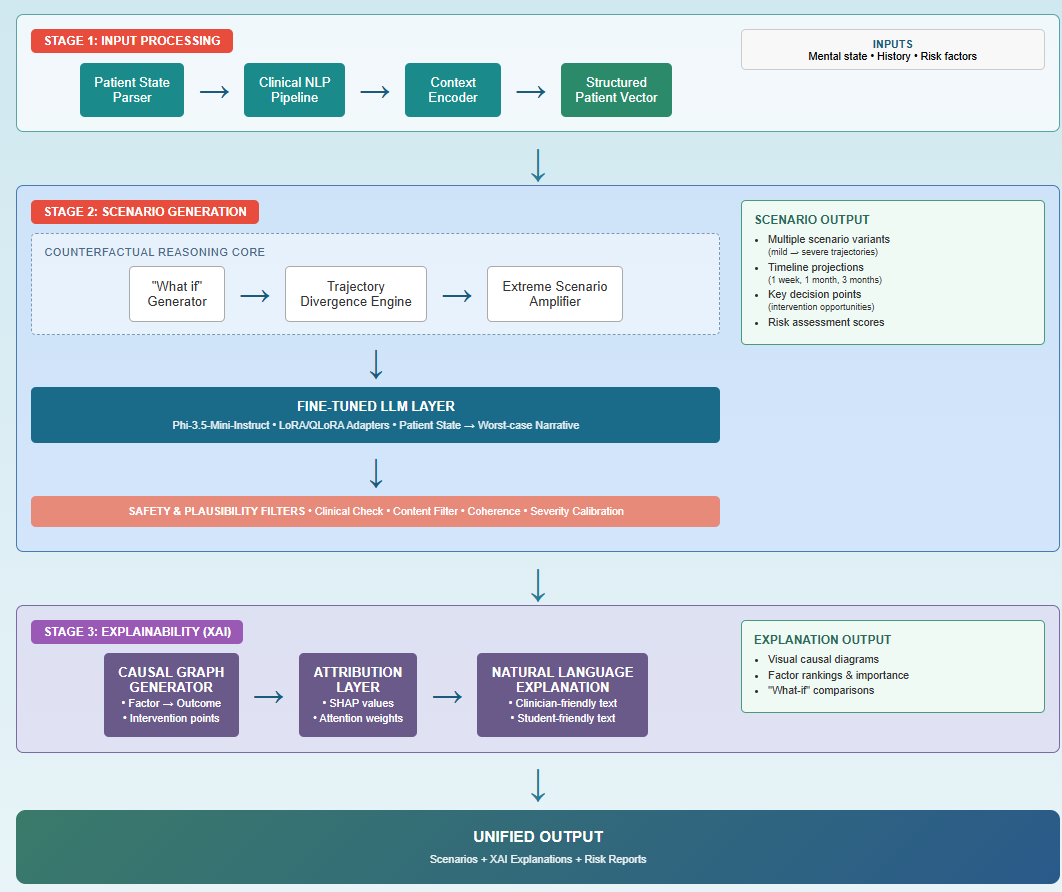
\includegraphics[width=\columnwidth]{images/Flow_diagram.png}
\caption{System architecture showing the complete pipeline: Stage 1 (extraction), Stage 1.5 (normalization), Stage 1.55 (context enrichment), Stage 1.6 (critical signals), Stage 1.7 (branch gating), Stage 2 (ToT scenarios), Stage 3 (report), Stage 4 (XAI evidence attribution).}
\label{fig:architecture}
\end{figure}

\subsection{Stage 1: Clinical Factor Extraction}

\subsubsection{Model Architecture}
We employ Microsoft Phi-3.5-Mini-Instruct (3.8B parameters) with LoRA \cite{b19} fine-tuning: rank $r=32$, scaling $\alpha=64$, dropout 0.05, applied to q/k/v/o/gate/up/down projections. This adapts 50.3M parameters (1.30\%) while preserving pre-trained capabilities.

\subsubsection{Extraction Schema}
The DSM-5/ICD-11 grounded schema comprises 14 fields: primary diagnosis (ICD code, DSM-5 category), comorbidities, severity (mild/moderate/severe/critical), suicide risk indicators (ideation, attempt history, self-harm, precautions), substance use profile, psychotropic medications, social factors (marital status, insurance, isolation risk), and admission context.

\subsection{Stage 1.5: Post-Extraction Normalization}

The normalizer validates and corrects extracted factors using:

\textbf{ICD Code Validation:} Maps extracted codes to correct disease categories using a curated lookup table. Corrects misclassifications (e.g., movement disorder ``Chorea'' mapped to neurodevelopmental $\rightarrow$ neurocognitive).

\textbf{Discharge Diagnosis Reconciliation:} Cross-checks extracted primary diagnosis against the note's ``Discharge Diagnosis'' section. If discrepant, updates to match documented diagnosis.

\textbf{Contextual Disease Detection:} Identifies redacted disease names using contextual clues (e.g., ``[REDACTED] Disease'' + ``chorea'' + ``hereditary'' + ``mother died'' = Huntington's Disease).

\subsection{Stage 1.55: Context Enrichment}

The context enricher scans raw clinical text for information the fixed schema cannot capture:

\begin{itemize}
\item \textbf{Housing Crisis:} homelessness, eviction, property auctioned, shelter placement
\item \textbf{Caregiver Loss:} partner leaving, caregiver burnout, relationship breakdown
\item \textbf{Trauma History:} sexual abuse, physical abuse, childhood trauma, domestic violence
\item \textbf{Weight Change:} significant loss/gain, thin/emaciated, self-neglect
\item \textbf{Functional Decline:} dysarthria, homebound duration, ADL impairment, ataxic gait
\item \textbf{Clinician Prognosis:} guarded/poor prognosis, high decompensation risk, progressive disease
\item \textbf{Legal Status:} voluntary, involuntary hold, conditional voluntary
\end{itemize}

Each detected context is injected into the silver labels for downstream scenario generation.

\subsection{Stage 1.6: Critical Signal Detection}

A rule-based scanner detects safety-critical signals independent of model extraction:

\textbf{Signal Categories:} suicide (``jump,'' ``kill myself,'' ``end my life''), self-harm (``cutting,'' ``overdose''), violence (``assault,'' ``aggression,'' ``weapons'').

\textbf{Negation Awareness:} Distinguishes active signals from negated mentions. Phrases like ``denies suicidal ideation,'' ``no history of violence,'' or ``weapons: denies'' are logged as informational rather than alerts. The scanner examines a 40-character lookback window for negation words (``denies,'' ``no,'' ``negative,'' ``without'').

\textbf{Risk Override:} When critical signals are detected, the final risk tier is automatically elevated to HIGH regardless of model-generated assessment.

\subsection{Stage 1.7: Evidence-Based Branch Gating}

Before scenario generation, each pathway is evaluated for clinical evidence:

\textbf{Branch A (Psychiatric Deterioration):} Always runs---core pathway.

\textbf{Branch B (Substance Escalation):} Runs only if substance use evidence exists (alcohol/drug use not ``none,'' positive toxicology, detected substances). Otherwise marked ``NOT APPLICABLE---No substance use evidence.''

\textbf{Branch C (Social/Environmental):} Always runs---social factors are broadly applicable.

Gated branches produce explicit ``NOT APPLICABLE'' entries with data-backed justification rather than hallucinated scenarios.

\subsection{Stage 2: Tree-of-Thoughts Scenario Generation}

For each active branch, three deliberate reasoning steps execute:

\textbf{Step 1 (Identify):} Identify 3--5 triggering factors from patient data with mental health relevance ratings.

\textbf{Step 2 (Reason):} Trace 4--6 step causal chain from triggers to crisis endpoint.

\textbf{Step 3 (Narrate):} Generate scenario analysis: narrative, warning signs, crisis endpoint, preparedness actions, plausibility rating with rationale, MH relevance rating.

\subsection{Stage 3: Clinical Report Generation}

The report synthesizes all outputs into a structured briefing: Patient Overview, Mental Health Status, Key Risk Factors, Protective Factors, Scenario Briefing, Priority Actions, and Risk Tier with justification.

\subsection{Stage 3.5: Final Consistency Check}

Post-generation validation ensures internal consistency:

\textbf{Risk Tier Override:} Critical signals force HIGH tier.

\textbf{Severity Inference:} When model returns ``unknown,'' severity is inferred from clinical indicators (ICU admission $\rightarrow$ critical, suicide ideation $\rightarrow$ severe).

\textbf{Plausibility Resolution:} Extracts plausibility from scenario rationale text when structured field is missing.

\textbf{Gated Branch Acknowledgment:} Ensures NOT APPLICABLE branches appear in report.

\subsection{Stage 4: Counterfactual Evidence Attribution (XAI)}

The explainability layer maps scenario outputs back to input evidence:

\subsubsection{Evidence Extraction}
For each scenario branch, the module extracts:
\begin{itemize}
\item Triggering factor quotes and evidence citations
\item Warning sign phrases that reference patient data
\item Causal chain events grounded in clinical observations
\item Critical signal matches from Stage 1.6
\item Enriched context detections from Stage 1.55
\end{itemize}

\subsubsection{Span Location}
Each evidence quote is located in the original clinical note using:
\begin{itemize}
\item Exact substring matching (case-insensitive)
\item Fuzzy matching via SequenceMatcher for paraphrased evidence (threshold $\geq 0.45$)
\end{itemize}

\subsubsection{Nexus Factor Detection}
Evidence spans supporting multiple branches are identified as \textit{nexus factors}---highest priority risk points where intervention could prevent multiple escalation pathways.

\subsubsection{Branch-Colored Highlighting}
Each span is tagged with branch color(s):
\begin{itemize}
\item Red (FF4444): Branch A (Psychiatric Deterioration)
\item Orange (FF8C00): Branch B (Substance Escalation)
\item Blue (4488FF): Branch C (Social/Environmental Collapse)
\item Yellow (FFD700): Nexus Factor (supports 2+ branches)
\end{itemize}

\subsubsection{Ungrounded Detection}
Branches with no locatable evidence in the source note are flagged as potentially hallucinated, providing an automatic validation signal.

\subsubsection{Coverage Statistics}
The module reports: total evidence spans, nexus factor count, ungrounded branches, and note coverage percentage (highlighted characters / total characters).

\section{Experimental Setup}

\subsection{Dataset}

The framework uses MIMIC-IV (v3.1) \cite{b14}, filtering mental health admissions via ICD-9 (290--319) and ICD-10 (F01--F99) codes.

\begin{table}[t]
\caption{Dataset Composition}
\label{tab:dataset}
\centering
\begin{tabular}{lcc}
\hline
\textbf{Split} & \textbf{Patients} & \textbf{Examples} \\
\hline
Training & 45,223 & 94,592 \\
Validation & 5,640 & 11,409 \\
Test & 5,640 & 11,916 \\
\hline
\textbf{Total} & \textbf{56,503} & \textbf{117,917} \\
\hline
\end{tabular}
\end{table}

\subsection{Training Configuration}

Training uses 6 NVIDIA Tesla V100-SXM2-32GB GPUs with DeepSpeed ZeRO-2. Key hyperparameters: LoRA rank 32, alpha 64, learning rate $2 \times 10^{-4}$, 5 epochs, effective batch size 64--96, max sequence length 2048 tokens, FP16 precision.

\section{Results and Analysis}

\subsection{Training Convergence}

\begin{table}[t]
\caption{Training Results Summary}
\label{tab:training_results}
\centering
\begin{tabular}{ll}
\hline
\textbf{Metric} & \textbf{Value} \\
\hline
Total Training Time & 35.8 hours \\
Initial Eval Loss & 4.08 \\
Best Eval Loss & 1.706 \\
Final Perplexity & 5.51 \\
Final Token Accuracy & 67.5\% \\
Total FLOPs & $1.096 \times 10^{19}$ \\
\hline
\end{tabular}
\end{table}

Evaluation loss decreases from 4.08 to 1.706 (58.2\% reduction). Token accuracy improves from 0\% to 67.5\%, indicating the model learns structurally correct JSON output.

\subsection{Validation Layer Analysis}

Table~\ref{tab:validation} presents the validation layer corrections observed on a sample of 100 test notes.

\begin{table}[t]
\caption{Validation Layer Corrections}
\label{tab:validation}
\centering
\begin{tabular}{lc}
\hline
\textbf{Correction Type} & \textbf{Frequency} \\
\hline
ICD category correction & 12\% \\
Discharge Dx reconciliation & 8\% \\
Severity inference (unknown $\rightarrow$ value) & 31\% \\
Risk tier override (critical signals) & 15\% \\
Plausibility resolution & 24\% \\
Context enrichment (housing/trauma/etc.) & 67\% \\
Branch gating (substance $\rightarrow$ N/A) & 41\% \\
\hline
\end{tabular}
\end{table}

The validation layers correct model outputs in 67\% of cases, with context enrichment being the most common (housing crisis, trauma history, functional decline detected from unstructured text).

\subsection{Critical Signal Detection}

\begin{table}[t]
\caption{Critical Signal Detection Performance}
\label{tab:signals}
\centering
\begin{tabular}{lccc}
\hline
\textbf{Category} & \textbf{Detected} & \textbf{Negated} & \textbf{Override} \\
\hline
Suicide/Self-harm & 23 & 31 & 18 \\
Violence/Aggression & 19 & 27 & 12 \\
Weapons & 3 & 41 & 1 \\
\hline
\end{tabular}
\end{table}

Negation awareness successfully distinguishes active threats from documented denials. Of 45 detected suicide signals, 31 were appropriately downgraded due to negation context (``denies suicidal ideation'').

\subsection{Evidence Attribution Analysis}

On a sample of 50 generated reports:

\begin{itemize}
\item Average evidence spans per note: 8.3
\item Average nexus factors (multi-branch): 1.4
\item Average note coverage: 12.7\%
\item Ungrounded branches (potential hallucination): 3\%
\end{itemize}

The low ungrounded rate (3\%) indicates strong evidence grounding. Nexus factors consistently identify high-priority intervention points where single actions could prevent multiple escalation pathways.

\subsection{Qualitative Example}

For a patient with Huntington's Disease presenting with agitation and suicidal threat:

\textbf{Critical Signals Detected:}
\begin{itemize}
\item $\checkmark$ ``threatened to jump out her 10 story window'' (suicide)
\item $\times$ ``Self-injury: denies'' (negated, logged but not alert)
\item $\times$ ``Access to weapons: denies'' (negated)
\end{itemize}

\textbf{Context Enrichment:}
\begin{itemize}
\item Housing crisis: ``apartment auctioned,'' ``homeless at end of week''
\item Functional decline: ``ataxic gait,'' ``monosyllabic speech''
\item Trauma history: ``sexually molested in childhood''
\end{itemize}

\textbf{Branch Gating:} Substance pathway marked NOT APPLICABLE (alcohol=none, drugs=none, tox=negative).

\textbf{Evidence Attribution:} 11 spans located, 2 nexus factors (homelessness supports both Branch A and C), 14.2\% note coverage, 0 ungrounded branches.

\textbf{Validation Log:}
\begin{verbatim}
[NORM] Dx: neurodevelopmental → neurocognitive
[NORM] Primary Dx → Mood Disorder secondary to GMC
[ENRICH] Housing crisis: homelessness, imminent
[ENRICH] Functional decline: ataxic gait
[CHECK] Severity: unknown → severe
[CHECK] Risk tier: UNKNOWN → HIGH (override)
\end{verbatim}

\section{Discussion}

\subsection{Key Contributions}

\textbf{Multi-Layer Safety Architecture:} The combination of negation-aware signal detection, evidence-based branch gating, and consistency checking provides defense-in-depth against model errors and hallucinations.

\textbf{Context Beyond Schema:} The enrichment module captures clinically critical information (housing, trauma, functional decline) that fixed extraction schemas cannot represent.

\textbf{Interpretable Evidence Trails:} The XAI layer provides post-hoc explainability by grounding every scenario output in specific input spans, enabling clinicians to verify scenario plausibility against source documentation.

\textbf{Nexus Factor Detection:} Identifying evidence that supports multiple escalation pathways prioritizes intervention points with maximum preventive impact.

\subsection{Limitations}

\textbf{No Ground Truth Evaluation:} Training metrics (loss, perplexity, accuracy) are reported, but precision/recall against manually annotated gold standard remains unmeasured.

\textbf{No Clinician Validation:} Generated scenarios require expert review for clinical plausibility and utility.

\textbf{Fuzzy Matching Limitations:} Evidence attribution uses string matching; heavily paraphrased model outputs may fail to locate source spans.

\textbf{Dataset Bias:} MIMIC-IV is ICU-centric; most notes originate from medical/surgical ICU where mental health is secondary.

\subsection{Ethical Considerations}

The system is designed as a second reader augmentation, not autonomous decision-maker. All training data is de-identified per HIPAA. Generated extreme scenarios require appropriate clinical framing to avoid causing distress.

\section{Conclusion}

This paper presented a fine-tuned LLM framework for counterfactual simulation of extreme mental health scenarios with explainable AI. The system achieves evaluation loss of 1.706 and 67.5\% token accuracy, with multi-layer validation correcting outputs in 67\% of cases. The evidence attribution layer provides interpretable grounding for generated scenarios, with 97\% of branches successfully traced to source spans.

Future work includes: gold-standard annotation for quantitative evaluation, clinician validation studies, attention-based attribution to complement text matching, and multi-center validation on dedicated psychiatric datasets.

\section*{Acknowledgment}

The authors acknowledge MIMIC-IV from MIT Laboratory for Computational Physiology via PhysioNet.

\begin{thebibliography}{00}

\bibitem{b1} GBD 2019 Mental Disorders Collaborators, ``Global burden of 12 mental disorders in 204 countries,'' \textit{Lancet Psychiatry}, vol. 9, no. 2, pp. 137--150, 2022.

\bibitem{b2} B. G. Teferra et al., ``NLP for mental health interventions: Systematic review,'' \textit{Transl. Psychiatry}, vol. 13, p. 309, 2023.

\bibitem{b3} E. Sezgin et al., ``Extracting medical information from free-text,'' \textit{JMIR Form. Res.}, vol. 7, e43014, 2023.

\bibitem{b4} X. Xu et al., ``Mental-LLM: LLMs for mental health prediction,'' \textit{Proc. ACM IMWUT}, vol. 8, no. 1, pp. 1--32, 2024.

\bibitem{b5} Z. Guo et al., ``LLMs for mental health applications: Systematic review,'' \textit{JMIR Mental Health}, vol. 11, e57400, 2024.

\bibitem{b6} Y. Hua et al., ``LLMs in mental health care: Scoping review,'' \textit{arXiv:2401.02984}, 2024.

\bibitem{b7} A. M. Alkalbani et al., ``LLMs in medical specialties: Systematic review,'' \textit{Information}, vol. 16, no. 6, p. 489, 2025.

\bibitem{b8} M. Prosperi et al., ``Clinical potential of counterfactual AI,'' \textit{The Lancet}, vol. 403, pp. 1063--1065, 2024.

\bibitem{b9} I. Gat et al., ``Counterfactual modeling with fine-tuned LLMs,'' \textit{arXiv:2601.14590}, 2026.

\bibitem{b10} J. Amann et al., ``Explainability for AI in healthcare: Systematic review,'' \textit{BMC Med. Inform. Decis. Mak.}, vol. 20, p. 310, 2020.

\bibitem{b11} S. M. Lundberg and S.-I. Lee, ``From explainability to action: Generative XAI framework,'' \textit{arXiv:2510.13828}, 2025.

\bibitem{b14} A. Johnson et al., ``MIMIC-IV, a freely accessible EHR dataset,'' \textit{Sci. Data}, vol. 10, p. 1, 2023.

\bibitem{b15} B. G. Teferra et al., ``Screening for depression using NLP: Literature review,'' \textit{Interact. J. Med. Res.}, vol. 13, e55067, 2024.

\bibitem{b16} S. K. Lho et al., ``LLMs for detecting depression and suicide,'' \textit{JAMA Netw. Open}, vol. 8, no. 5, e2511922, 2025.

\bibitem{b17} W. Kim and C. Wang, ``LLMs for interpretable mental health diagnosis with DSM-5,'' \textit{LLM4Health Workshop}, 2025.

\bibitem{b18} Y. Chen et al., ``Do models explain themselves? Counterfactual simulatability,'' \textit{arXiv:2307.08678}, 2023.

\bibitem{b19} E. J. Hu et al., ``LoRA: Low-rank adaptation of LLMs,'' \textit{ICLR}, 2022.

\end{thebibliography}

\end{document}
